% questions.tex —— 2006 年·上海春季招生数学试卷 · 题目内容片段（无答案）
% 由 tools/generate_projects.py 依来源总账自 2006/2006_数学真题_春季上海_试题.md 生成，勿手改（改源 MD 后重跑）


\begin{gktip}
\textbf{来源边界}：题面依据固定 PDF 第 1–2 页转录。固定扫描件页眉标有《数学教学》2006 年第 2 期，印刷页码 2-39 至 2-42；现有证据只固定此扫描副本及其内部题签，杂志出版信息、扫描来源链与题面/答案的官方身份尚未核实。第 2–4 页印有“参考答案”及解答，本题面稿不混入源载答案，也不据此称答案为官方答案。
\end{gktip}

\gkpart{一、填空题}

（本大题满分 48 分，共 12 题，每题填对得 4 分，否则得零分。）

\begin{question}
\gkti{1}计算：$\displaystyle\lim_{n\to\infty}\frac{3n-2}{4n+3}=\underline{\qquad}$。

\end{question}
\begin{question}
\gkti{2}方程 $\log_3(2x-1)=1$ 的解 $x=\underline{\qquad}$。

\end{question}
\begin{question}
\gkti{3}函数 $f(x)=3x+5$，$x\in[0,1]$ 的反函数 $f^{-1}(x)=\underline{\qquad}$。

\end{question}
\begin{question}
\gkti{4}不等式 $\displaystyle\frac{1-2x}{x+1}>0$ 的解集是 $\underline{\qquad}$。

\end{question}
\begin{question}
\gkti{5}已知圆 $C:(x+5)^2+y^2=r^2\ (r>0)$ 和直线 $l:3x+y+5=0$。若圆 $C$ 与直线 $l$ 没有公共点，则 $r$ 的取值范围是 $\underline{\qquad}$。

\end{question}
\begin{question}
\gkti{6}已知函数 $f(x)$ 是定义在 $(-\infty,+\infty)$ 上的偶函数。当 $x\in(-\infty,0)$ 时，$f(x)=x-x^4$，则当 $x\in(0,+\infty)$ 时，$f(x)=\underline{\qquad}$。

\end{question}
\begin{question}
\gkti{7}电视台连续播放 6 个广告，其中含 4 个不同的商业广告和 2 个不同的公益广告，要求首尾必须播放公益广告，则共有 $\underline{\qquad}$ 种不同的播放方式（结果用数值表示）。

\end{question}
\begin{question}
\gkti{8}正四棱锥底面边长为 4，侧棱长为 3，则其体积为 $\underline{\qquad}$。

\end{question}
\begin{question}
\gkti{9}在 $\triangle ABC$ 中，已知 $BC=8$，$AC=5$，三角形面积为 12，则 $\cos 2C=\underline{\qquad}$。

\end{question}
\begin{question}
\gkti{10}若向量 $\vec a,\vec b$ 的夹角为 $150^\circ$，$|\vec a|=\sqrt3$，$|\vec b|=4$，则 $|2\vec a+\vec b|=\underline{\qquad}$。

\end{question}
\begin{question}
\gkti{11}已知直线 $l$ 过点 $P(2,1)$，且与 $x$ 轴、$y$ 轴的正半轴分别交于 $A\text{、}B$ 两点，$O$ 为坐标原点，则三角形 $OAB$ 面积的最小值为 $\underline{\qquad}$。

\end{question}
\begin{question}
\gkti{12}同学们都知道，在一次考试后，如果按顺序去掉一些高分，那么班级的平均分将降低；反之，如果按顺序去掉一些低分，那么班级的平均分将提高。这两个事实可以用数学语言描述为：若有限数列 $a_1,a_2,\cdots,a_n$ 满足 $a_1\leq a_2\leq\cdots\leq a_n$，则
\nopagebreak[4]
\[
\frac{a_1+a_2+\cdots+a_m}{m}\leq\frac{a_1+a_2+\cdots+a_n}{n}\leq\frac{a_{m+1}+a_{m+2}+\cdots+a_n}{n-m}\quad(1\leq m<n).
\]
（结论用数学式子表示。）

\end{question}
\gkpart{二、选择题}

（本大题满分 16 分，共 4 题，每题 4 分。每题给出四个结论，其中有且只有一个结论是正确的，必须把正确结论的代号写在题后的圆括号内，选对得 4 分，否则得零分。）

\begin{question}
\gkti{13}抛物线 $y^2=4x$ 的焦点坐标为\mbox{（　　）}。

（A）$(0,1)$　　（B）$(1,0)$　　（C）$(0,2)$　　（D）$(2,0)$

\end{question}
\begin{question}
\gkti{14}若 $a,b,c\in\mathbb R$，$a>b$，则下列不等式成立的是\mbox{（　　）}。

（A）$\displaystyle\frac1a<\frac1b$　　（B）$a^2>b^2$

（C）$\displaystyle\frac{a}{c^2+1}>\frac{b}{c^2+1}$　　（D）$a|c|>b|c|$

\end{question}
\begin{question}
\gkti{15}若 $k\in\mathbb R$，则“$k>3$”是“方程
\nopagebreak[4]
\[
\frac{x^2}{k-3}-\frac{y^2}{k+3}=1
\]
表示双曲线”的\mbox{（　　）}。

（A）充分不必要条件　　（B）必要不充分条件

（C）充要条件　　（D）既不充分也不必要条件

\end{question}
\begin{question}
\gkti{16}若集合
\nopagebreak[4]
\[
A=\left\{y\mid y=x^{\frac13},\ -1\leq x\leq1\right\},\qquad
B=\left\{y\mid y=2-\frac1x,\ 0<x\leq1\right\},
\]
则 $A\cap B$ 等于\mbox{（　　）}。

（A）$(-\infty,1]$　　（B）$[-1,1]$　　（C）$\varnothing$　　（D）$\{1\}$

\end{question}
\gkpart{三、解答题}

（本大题满分 86 分，共 6 题，解答下列各题必须写出必要的步骤。）

\Needspace{0.4\textheight}
\begin{question}
\gkti{17}\textbf{（本题满分 12 分）} 

在长方体 $ABCD-A_1B_1C_1D_1$ 中，已知 $DA=DC=4$，$DD_1=3$，求异面直线 $A_1B$ 与 $B_1C$ 所成角的大小（结果用反三角函数值表示）。
\nopagebreak[4]
\begin{center}% 2006 年上海春季卷第 17 题：长方体及题干指定的两条异面直线。
% 只示意原卷可见拓扑与虚实线，不按比例，不暗示边长比例。
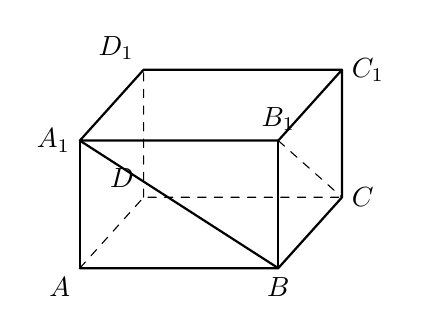
\begin{tikzpicture}[line cap=round,line join=round,scale=0.9]
  \coordinate (A) at (0,0);
  \coordinate (B) at (2.8,0);
  \coordinate (C) at (3.7,1.0);
  \coordinate (D) at (0.9,1.0);
  \coordinate (A1) at (0,1.8);
  \coordinate (B1) at (2.8,1.8);
  \coordinate (C1) at (3.7,2.8);
  \coordinate (D1) at (0.9,2.8);

  % 长方体可见棱与遮挡棱。
  \draw[thick] (A)--(B)--(C)--(C1)--(B1)--(A1)--(D1)--(C1);
  \draw[thick] (A1)--(A) (B1)--(B);
  \draw[dashed] (A)--(D)--(C) (D)--(D1);

  % 题干中的 A_1B 与 B_1C。
  \draw[thick] (A1)--(B);
  \draw[dashed] (B1)--(C);

  \node[below left] at (A) {$A$};
  \node[below] at (B) {$B$};
  \node[right] at (C) {$C$};
  \node[above left] at (D) {$D$};
  \node[left] at (A1) {$A_1$};
  \node[above] at (B1) {$B_1$};
  \node[right] at (C1) {$C_1$};
  \node[above left] at (D1) {$D_1$};
\end{tikzpicture}
\end{center}
\nopagebreak[4]
\end{question}
\begin{question}
\gkti{18}\textbf{（本题满分 12 分）} 

已知复数 $w$ 满足 $w-4=(3-2w)i$（$i$ 为虚数单位），$z=\dfrac5w+|w-2|$，求一个以 $z$ 为根的实系数一元二次方程。

\end{question}
\begin{question}
\gkti{19}\textbf{（本题满分 14 分）} 本题共有 2 个小题，第 1 小题满分 8 分，第 2 小题满分 6 分。

\Needspace{5\baselineskip}
已知函数
\nopagebreak[4]
\[
f(x)=2\sin\left(x+\frac\pi6\right)-2\cos x,\qquad x\in\left[\frac\pi2,\pi\right].
\]

（1） 若 $\sin x=\dfrac45$，求函数 $f(x)$ 的值；

（2） 求函数 $f(x)$ 的值域。

\Needspace{0.4\textheight}
\end{question}
\begin{question}
\gkti{20}\textbf{（本题满分 14 分）} 本题共有 2 个小题，第 1 小题满分 6 分，第 2 小题满分 8 分。

学校科技小组在计算机上模拟航天器变轨返回试验。设计方案如图：航天器运行（按顺时针方向）的轨迹方程为 $\dfrac{x^2}{100}+\dfrac{y^2}{25}=1$，变轨（即航天器运行轨迹由椭圆变为抛物线）后返回的轨迹是以 $y$ 轴为对称轴、$M\left(0,\dfrac{64}{7}\right)$ 为顶点的抛物线的实线部分，降落点为 $D(8,0)$。观测点 $A(4,0)\text{、}B(6,0)$ 同时跟踪航天器。
\nopagebreak[4]
\begin{center}% 2006 年上海春季卷第 20 题：原卷航天器轨迹示意图的矢量重绘。
% 曲线按题设方程绘制；原图为示意图，除题干已给坐标外不引入比例条件。
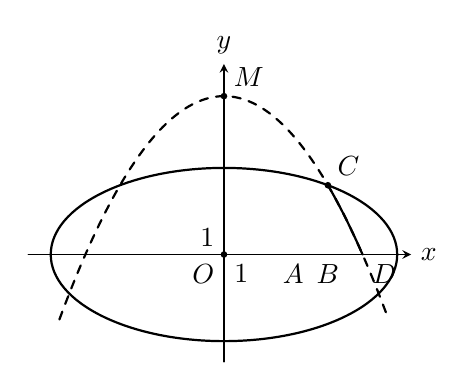
\begin{tikzpicture}[line cap=round,line join=round,x=0.22cm,y=0.22cm,>=stealth]
  % 坐标轴与椭圆运行轨迹 x^2/100+y^2/25=1。
  \draw[->] (-11.3,0)--(10.8,0) node[right] {$x$};
  \draw[->] (0,-6.2)--(0,11.0) node[above] {$y$};
  \draw[thick] (0,0) ellipse (10 and 5);

  % 变轨后的抛物线 y=64/7-x^2/7，原卷以虚线表示。
  \draw[dashed,thick,domain=-9.5:9.5,samples=100,variable=\x]
    plot (\x,{64/7-\x*\x/7});
  % 原卷以实线强调从交点 C 到降落点 D 的运行弧段。
  \draw[thick,domain=6:8,samples=40,variable=\x]
    plot (\x,{64/7-\x*\x/7});

  % 原卷中的基准点与观测点标记。
  \fill (0,0) circle (1.2pt) node[below left] {$O$};
  \fill (0,{64/7}) circle (1.2pt) node[above right] {$M$};
  \fill (6,4) circle (1.2pt) node[above right] {$C$};
  \node[below] at (4,0) {$A$};
  \node[below] at (6,0) {$B$};
  \node[below right] at (8,0) {$D$};
  \node[below] at (1,0) {$1$};
  \node[left] at (0,1) {$1$};
\end{tikzpicture}
\end{center}
\nopagebreak[4]
（1） 求航天器变轨后的运行轨迹所在的曲线方程；

（2） 试问：当航天器在 $x$ 轴上方时，观测点 $A\text{、}B$ 测得离航天器的距离分别为多少时，应向航天器发出变轨指令？

\Needspace{0.4\textheight}
\end{question}
\begin{question}
\gkti{21}\textbf{（本题满分 16 分）} 本题共有 3 个小题，第 1 小题满分 4 分，第 2 小题满分 6 分，第 3 小题满分 6 分。

设函数 $f(x)=|x^2-4x-5|$。

（1） 在区间 $[-2,6]$ 上画出函数 $f(x)$ 的图象；

（2） 设集合 $A=\{x\mid f(x)\geq5\}$，$B=(-\infty,-2]\cup[0,4]\cup[6,+\infty)$。试判断集合 $A$ 和 $B$ 之间的关系，并给出证明；

（3） 当 $k>2$ 时，求证：在区间 $[-1,5]$ 上，$y=k(x+3)$ 的图象位于函数 $f(x)$ 图象的上方。
\nopagebreak[4]
\begin{center}% 2006 年上海春季卷第 21 题：原卷留白坐标网格。
% 单位网格覆盖 [-10,10]×[-10,10]，坐标轴数字按原卷显示到偶数刻度。
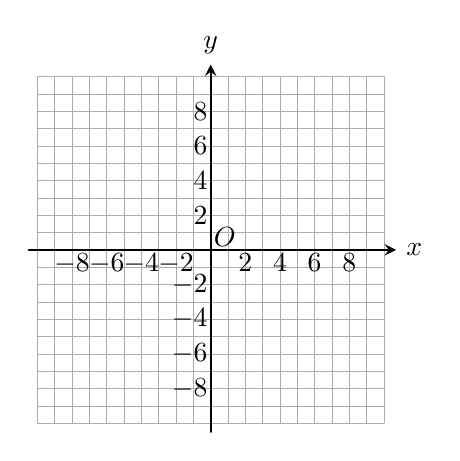
\begin{tikzpicture}[line cap=round,line join=round,x=0.22cm,y=0.22cm,>=stealth]
  \draw[step=1,gray!65,very thin] (-10,-10) grid (10,10);
  \draw[->,thick] (-10.5,0)--(10.7,0) node[right] {$x$};
  \draw[->,thick] (0,-10.5)--(0,10.7) node[above] {$y$};

  \foreach \x in {-8,-6,-4,-2,2,4,6,8}
    \node[below,inner sep=1pt] at (\x,0) {$\x$};
  \foreach \y in {-8,-6,-4,-2,2,4,6,8}
    \node[left,inner sep=1pt] at (0,\y) {$\y$};
  \node[above right,inner sep=1pt] at (0,0) {$O$};
\end{tikzpicture}
\end{center}
\nopagebreak[4]
\end{question}
\begin{question}
\gkti{22}\textbf{（本题满分 18 分）} 本题共有 3 个小题，第 1 小题满分 4 分，第 2 小题满分 8 分，第 3 小题满分 6 分。

已知数列 $a_1,a_2,\cdots,a_{30}$，其中 $a_1,a_2,\cdots,a_{10}$ 是首项为 1，公差为 1 的等差数列；$a_{10},a_{11},\cdots,a_{20}$ 是公差为 $d$ 的等差数列；$a_{20},a_{21},\cdots,a_{30}$ 是公差为 $d^2$ 的等差数列（$d\neq0$）。

（1） 若 $a_{20}=40$，求 $d$；

（2） 试写出 $a_{30}$ 关于 $d$ 的关系式，并求 $a_{30}$ 的取值范围；

（3） 续写已知数列，使得 $a_{30},a_{31},\cdots,a_{40}$ 是公差为 $d^3$ 的等差数列，……，依次类推，把已知数列推广为无穷数列。提出同（2）类似的问题（（2）应当作为特例），并进行研究，你能得到什么样的结论？

\end{question}